\documentclass{SGGW-thesis}
\graphicspath{ {./images/} }

\INZYNIERSKAtrue
\WZIMtrue

\listfiles

\title{Porównanie aplikacji frontendowych opartych na mikrofrontendach z tradycyjną architekturą monolityczną na przykładzie aplikacji do zarządzania finansami osobistymi}
\Etitle{Comparison of Microfrontend Applications and Monolith Frontend Applications Based on the Example of Expense Tracker}
\author{Dawid Wijata}
\date{2023}
\album{205006}
\thesis{Praca dyplomowa na kierunku:}
\course{Informatyka}
\promotor{dr. \ inż.\ Piotra Wrzeciono}
\pworkplace{Instytut Informatyki Technicznej\\Katedra Systemów Informacyjnych}

\raggedbottom

\begin{document}

% uniezależnienie numerów tabel, rysunków i listingów od rozdziału
\counterwithout{table}{chapter}
\counterwithout{figure}{chapter}
\counterwithout{lstlisting}{chapter}

\makeatother

\maketitle
\statementpage
\abstractpage
{Porównanie aplikacji frontendowych opartych na mikrofrontendach z tradycyjną architekturą monolityczną na przykładzie aplikacji do zarządzania finansami osobistymi}
{Tematem niniejszej pracy była implementacja i poźniejsze porównanie frontendu dwóch wersji aplikacji do zarządzania finansami osobistymi w dwóch architekturach - mikrofrontendowej i monolitycznej. Praca składa się z części teoretycznej wprowadzającej w pojęcie mikroserwisów i mikrofrontendów oraz części praktycznej porównującej obie implementacje pod względem metryk kodu, wydajności, kosztów obu rozwiązań oraz zarządzania projektem.}
{architektura rozproszona, mikroserwisy, mikrofrontendy, architektura oprogramowania}
{Comparison of Microfrontend Applications and Monolith Frontend Applications Based on the Example of Expense Tracker}
{The subject of this thesis was to implement and compare frontend parts of expense tracker web application written in two different architectural concepts - monolith and microfrontends. The first part is an introduction to microservice and microfrontend concepts. The second one consists of a comparison of both application versions by terms of code metrics, performance, financial costs of both solutions and project management.}
{distributed architecture, microservices, microfrontends, software architecture}

% Spis treści może być złożony z pojedynczą interlinią, np. jeśli jedna linia wychodzi na następną stronę.
% W przeciwnym razie spis treści wstawić bez powyższego rozkazu i klamry.
{
	\doublespacing
	\tableofcontents
}

\startchapterfromoddpage % niezależnie od długości spisu treści pierwszy rozdział zacznie się na nieparzystej stronie

\chapter{Wstęp}
Celem niniejszej pracy była implementacja i porównanie warstwy frontendowej aplikacji do zarządzania finansami w dwóch wersjach do zarządzania finansami osobistymi w dwóch architekturach - mikrofrontendowej i monolitycznej.

\section{Architektura monolityczna}
Monolitem, bądź programem zaprojektowanym zgodnie z architekturą monolityczną nazywamy program uruchamiany w całości za pomocą jednego pliku wykonywalnego. W~aplikacjach webowych taka architektura spełnia założenia modelu trójwarstwowego. Na te warstwy składają się:

\begin{enumerate}
	\item interfejs użytkownika składający się z dokumentów HTML, arkuszy styli CSS oraz skryptów JavaScript definiujących zachowanie interfejsu użytkownika,
	\item warstwa API przygotowująca dane podawane do interfejsu użytkownika w celu pokazania go użytkownikowi,
	\item warstwa dostępu do danych.
\end{enumerate}

Taką strukturę trójwarstwową możemy opisać diagramem z \cref{fig:monolith_diagram}

\begin{figure}[h]
	\centering
	\captionsetup{justification=centering}
	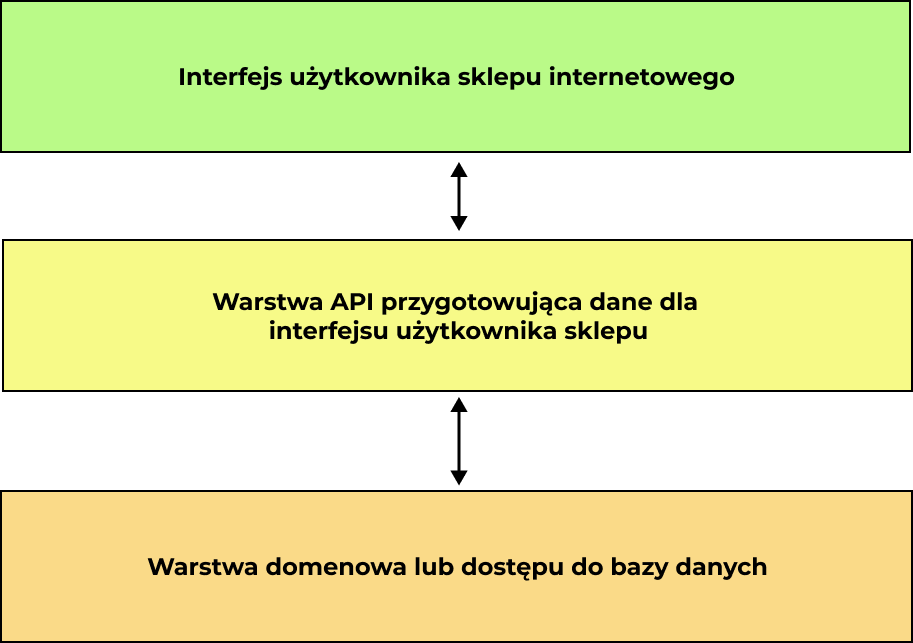
\includegraphics[width=0.75\textwidth]{monolith_diagram.png}
	\caption{Podział na warstwy dla przykładowego sklepu internetowego \\ w architekturze monolitycznej}
	\label{fig:monolith_diagram}
\end{figure}

Warstwa druga jest czasami pomijana przez twórców oprogramowania, co pozwala interfejsowi użytkownika na bezpośredni dostęp do danych. Różnicą między nimi jest brak istnienia warstwy oddzielającej logikę biznesową od interfejsu użytkownika. Wtedy możemy mówić o modelu dwuwarstwowym.
Wraz z rozwojem aplikacji w modelu dwuwarstwowym i trójwarstwowym oraz ciągłym dopisywaniu do nich nowych funkcjonalności, kod tych aplikacji stawał się coraz bardziej nieczytelny. Drzewo zależności między fragmentami kodu okazywały się być zbyt rozbudowane.
Ponadto każda zmiana w~oprogramowaniu powoduje konieczność zbudowania oraz wystawienia na środowisko produkcyjne kolejnej wersji oprogramowania. Przy dużych aplikacjach ten proces potrafi zabierać znaczącą ilość czasu. Utrudnia to też proces testowania oprogramowania, zarówno manualnie (ze względu na rosnącą ilość scenariuszy testowych) jak i automatycznie (ze względu na rosnący czas uruchomienia siatki testów).
Zgodnie z~pracą \cite{fowler}, pojęcia \textit{monolit} w~odniesieniu do oprogramowania pierwotnie używała społeczność programistów systemu operacyjnego Unix. Programiści Unix'a określali tak systemy, które stają się zbyt duże, by móc je komfortowo utrzymywać.

\section{Architektura mikroserwisów}

Trudności z utrzymaniem oprogramowania, które w obrębie jednego projektu zawiera ciągle rozrastającą się logikę, spowodowały konieczność zastosowania podziału kodu na mniejsze i jednocześnie prostsze w utrzymaniu części.
W związku z tym do większych aplikacji zaczęto stosować ich podział na części będące usługami niezależnymi od pozostałych elementów systemu. Taką pojedynczą usługę nazywamy mikroserwisem. Przykładowe rozmieszczenie modułów w projekcie mikroserwisowym możemy zaobserwować na \cref{fig:microservices_diagram}

\vfill
\clearpage

\begin{figure}[h]
	\centering
	\captionsetup{justification=centering}
	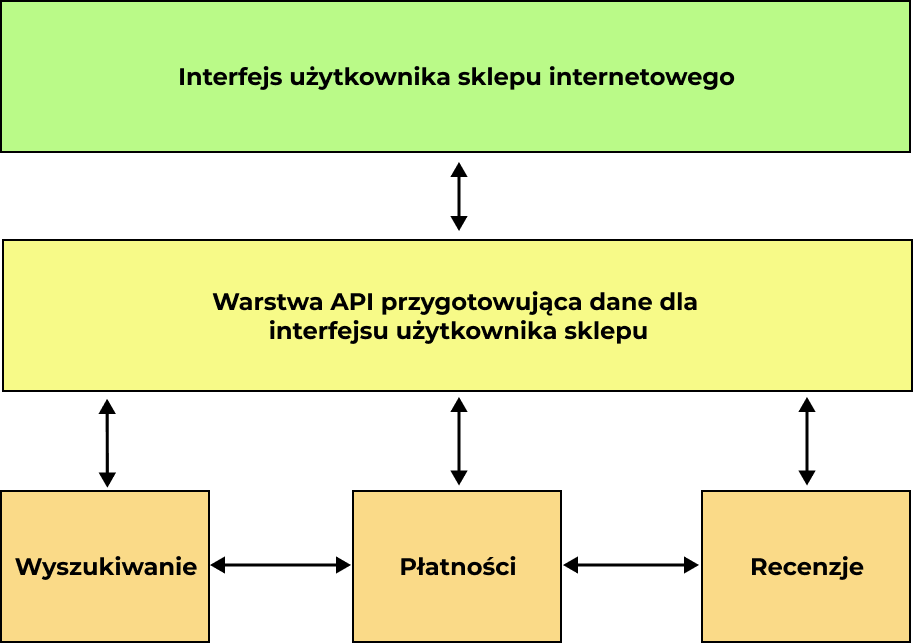
\includegraphics[width=0.8\textwidth]{microservices_diagram.png}
	\caption{Podział na moduły dla przykładowego sklepu internetowego \\ w architekturze mikroserwisowej}
	\label{fig:microservices_diagram}
\end{figure}


Komunikacja między mikroserwisami zachodzi przy użyciu protokołów sieciowych neutralnych w ujęciu technologicznym, na przykład HTTP. Podział aplikacji na serwisy pozwala na wykonywanie prac nad konkretnymi funkcjonalnościami aplikacji bez potencjalnego ryzyka naruszenia kodu odpowiedzialnego za inne funkcjonalności. Innymi zaletami tego rozwiązania są:

\begin{enumerate}
	\item dowolność w zastosowaniu technologii - pozwala na użycie do każdej funkcjonalności zasobów technologicznych najlepiej odpowiadających danemu zadaniu,
	\item stabilność - ewentualne problemy z aplikacją nie powodują zatrzymania całego systemu, a jedynie konkretnego serwisu,
	\item skalowalność - nowe funkcjonalności można dodawać poprzez dodanie nowych serwisów, a poszczególne serwisy można rozszerzać nie naruszając logiki innych serwisów,
	\item wzrost dostępności usług - w razie, gdyby któryś z serwisów przestał działać, inne usługi nadal będą dostępne.
\end{enumerate}

Przedstawione zalety są znaczące nie tylko z punktu widzenia projektowania i tworzenia oprogramowania, ale też z punktu zarządzania projektami. Jasny podział projektu na niezależne od siebie części pozwala też na przyporządkowanie ludzi do zespołów mniejszych, ale ściśle skoncentrowanych na konkretnym wycinku wiedzy potrzebnym do realizacji danej funkcjonalności.
Autonomiczność takich zespołów pozwala na zmniejszenie ilości potrzebnych kontaktów między zespołami w celu ustalenia rozwiązań problemów i dalszego przebiegu projektu. Pomaga to między innymi zmniejszyć ilość spotkań oraz skrócić te krytycznie potrzebne do realizacji projektu.

Rozrośnięcie się infrastruktury używającej mikroserwisów zwiększa też zapotrzebowanie na ludzi zajmujących się wsparciem developerów w zakresie konfiguracji infrastruktury (tzw. \textit{inżynierowie DevOps}), a w przypadku zastosowania technologii chmurowych, również specjalistów w zakresie technologii takich jak Microsoft Azure, Google Cloud oraz Amazon Web Services. Taka sytuacja również przyczynia się do zwiększenia kosztów związanych z oprogramowaniem w architekturze mikroserwisowej. Można jednak uznać ją za czynnik zmuszający firmy do rozwoju w~zakresie R\&D (\textit{Research and Development}) w celu ustalenia własnych standardów architektonicznych, które będą optymalne dla ich potrzeb biznesowych w zakresie realizacji mikroserwisów. Mimo to, czynniki kosztowe powodują, że wybór architektury mikroserwisowej do projektu może nie być optymalny dla małych i średnich projektów.

Mikroserwisy powodują też konieczność uzgodnienia konwencji między projektami w~sprawach takich jak:

\begin{itemize}
	\item postać wyjątków rzucanych przez serwisy,
	\item opis obiektów, które są częścią innych serwisów,
	\item sposób łączenia się między serwisami,
	\item autoryzacja i uwierzytelnianie,
	\item standard podziału kodu na projekty lub moduły.
\end{itemize}
Brak zgody między projektami w powyższych kwestiach może doprowadzić do jeszcze większego nieporządku, niż gdyby projekt był realizowany jako monolit. Ponadto, uporządkowana struktura projektu mikroserwisowego pozwala na replikowanie schematu na dowolną skalę, a co za tym idzie, automatyzację procesu tworzenia nowych serwisów. Można to zrealizować na przykład za pomocą szablonów projektu aplikowanych do środowiska programistycznego, obrazów środowiska Docker \cite{docker} lub idąc jeszcze dalej - odpowiednio ustawionym klastrze Kubernetes \cite{kubernetes}. Jednak przy sprostaniu tym wyzwaniom architektonicznym na etapie projektowania oprogramowania zyskamy dzięki mikroserwisom możliwość zarządzania projektem o dowolnej wielkości w sposób ściśle uporządkowany i z zachowaniem dobrej jakości kodu źródłowego oraz łatwe dostosowanie projektu do potrzeb biznesowych i metodologii zwinnych zarządzania projektami.

\chapter{Mikrofrontendy}
\section{Wstęp}
Pomimo zastosowania mikroserwisów przy projektowaniu logiki backendowej części aplikacji, frontendowa część projektu pozostawała w przeszłości mniej rozbudowana. Głównym powodem był fakt, że logika obliczeniowa i biznesowa występowała po stronie backendu. Odciążało to część frontendową, co pozwalało na mniejsze jej rozbudowanie oraz ograniczenie rozwarstwienia frontendu w postaci monolitu. Jednak wraz z rozwojem technologicznym w zakresie webowych interfejsów użytkownika, objętość kodu frontendowego w widoczny sposób wzrosła. Na taki stan rzeczy złożyło się wiele czynników takich jak:

\begin{itemize}
	\item powstawanie coraz bardziej kreatywnych i szczegółowych efektów wizualnych,
	\item optymalizacja działania skryptów JavaScript,
	\item zwiększająca się dojrzałość działalności programistów frontendu,
	\item rozwój frameworków strukturyzujących projekty frontendowe takich jak Angular \cite{angular}, React \cite{react}, Vue \cite{vue} (produkują one dziesiątki tysięcy linii kodu wynikowego).
\end{itemize}

Wszystkie te czynniki spowodowały potrzebę podzielenia kodu na pewnego rodzaju moduły. Najpopularniejsze frameworki radzą sobie jednak wystarczająco dobrze ze skutkami nagromadzenia dużej ilości kodu, aby używać ich w projektach komercyjnych. Najlepiej z tym problemem radzi sobie framework Angular, który proponuje programistom systemowy podział na moduły, oraz kilka propozycji na podziały niższego stopnia na struktury takie jak:

\begin{itemize}
	\item component,
	\item service,
	\item guard,
	\item pipe
	\item i inne.
\end{itemize}

Jednak struktura organizacyjna całego projektu oprogramowania różni się znacząco po stronie backendu, jak i frontendu. Może to powodować różne nieścisłości organizacyjne oraz zwiększać liczbę zapytań wykonanych między członkami zespołu w celu uzgodnienia szczegółów projektu. Zaczęto się więc rozglądać za sposobem organizacji pracy zespołu frontendowego takiego, żeby móc podzielić osoby pracujące nad projektem na zespoły w~pełni skoncentrowane na konkretnych funkcjonalnościach. Takie podejście zwiększa autonomiczność zespołów.
Takim sposobem okazało się być dostosowanie frontendowych części projektu do architektury mikroserwisowej. Zgodnie z rysunkiem \cref{fig:microfrontends_diagram} można podzielić zespół programistów frontendu na funkcjonalne grupy dostosowane do wcześniej utworzonych podzespołów tak, aby wynikowe podzespoły były już w~pełni skoncentrowane na wydzielonej partii wartości biznesowej.

\begin{figure}[h]
	\centering
	\captionsetup{justification=centering}
	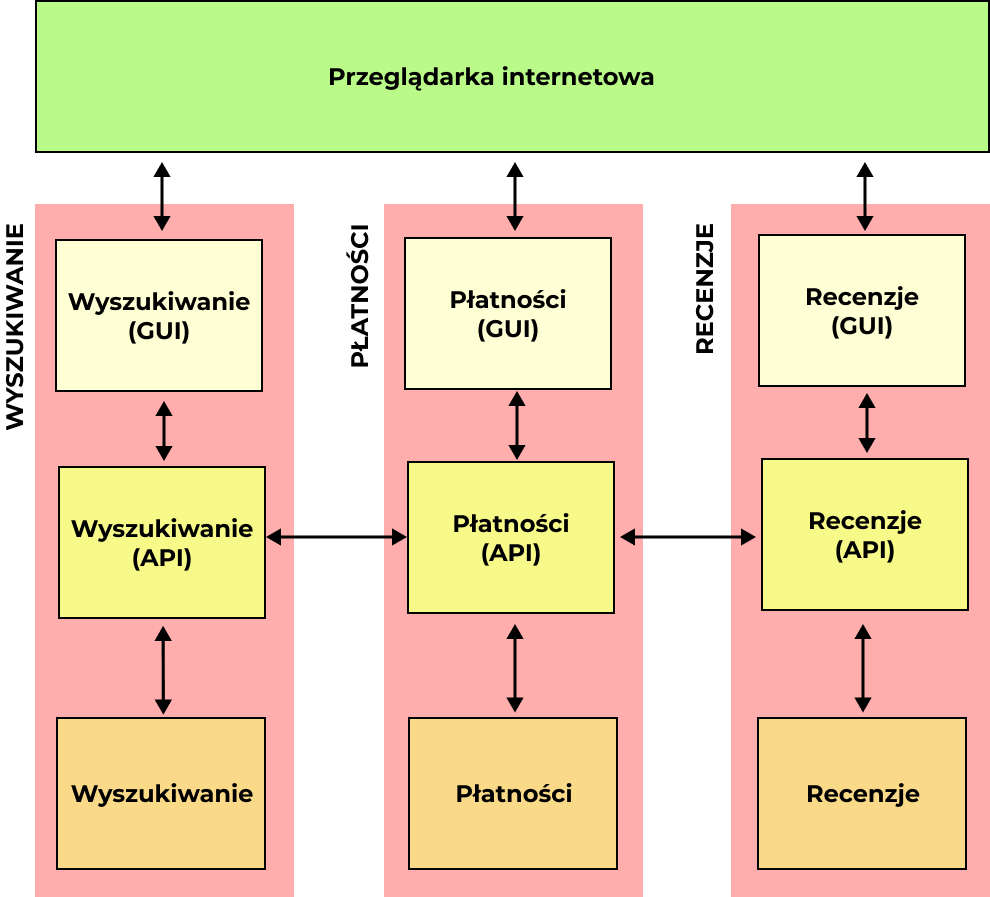
\includegraphics[width=0.8\textwidth]{microfrontends_diagram.png}
	\caption{Podział na moduły dla przykładowego sklepu internetowego \\ w architekturze mikrofrontendowej}
	\label{fig:microfrontends_diagram}
\end{figure}

Pojedynczą jednostkę funkcjonalną takiego podziału na frontendzie nazywamy \textit{mikrofrontendem}, a w ogólności architekturę używającą takiego podziału nazywamy architekturą mikrofrontendową.
Zgodnie z wynikami ankiety \cite{tsh_2022}, 24.6\% programistów biorących udział w ankiecie pracowało w 2021 roku w zespołach wykorzystujących w~projekcie architekturę mikrofrontendową. Ponadto, według tej ankiety, 37.2\% programistów biorących udział w ankiecie twierdzi, że w przeciągu dwóch następnych lat popularność koncepcji mikrofrontendów wzrośnie. Na podstawie tych statystyk można wnioskować, że pomysł rozszerzenia mikroserwisów na część frontendową przyjął się w~dużej części organizacji oraz przede wszystkim, w świadomości programistów.

\section{Dodatkowe ograniczenia względem mikroserwisów}
\subsection{Ograniczone zasoby obliczeniowe}
W przypadku prac nad backendowymi częściami projektu, coraz mniej zwraca się uwagę na optymalizację działania algorytmów używanych w oprogramowaniu. Pamięć operacyjna oraz masowa stały się dużo tańsze w przeliczeniu na jednostkę pamięci niż kilka lat temu. Dla klienta stało się tańsze zainwestowanie maksymalnie kilku tysięcy złotych na dołożenie pamięci do serwera, udostępniającego żądaną usługę sieciową, niż zainwestowanie wielokrotności tej kwoty w~czas pracy programistów, którzy zoptymalizują wadliwy algorytmicznie kod.
Nie ma to jednak zastosowania przy pracy nad frontendem. Przeglądarka, w której koniec końców efekty pracy są pokazane użytkownikowi końcowemu, oferuje jedynie swoje zasoby pamięci - nie można użyć tak dużego odsetka zasobów komputera, jak w przypadku backendu. Poza tym, minimalne odstępstwa od optymalizacji są zauważalne dla użytkownika końcowego. Każde przycięcie się elementów interfejsu, brak płynności powodują irytację użytkownika, a co dalej za tym idzie, spadek zadowolenia z używania wyprodukowanego oprogramowania. W przypadku zastosowania mikrofrontendów problem narasta. De facto ładujemy do przeglądarki jednocześnie kilka pełnoprawnych aplikacji i wymagamy od nich, aby one wszystkie podzieliły się niewielkimi zasobami pamięci i procesora zaalokowanymi przez przeglądarkę w taki sposób, aby każda z nich działała w sposób komfortowy dla użytkownika. Na szczęście rozwiązanie problemu jest konceptualnie bardzo proste. Wystarczy ładować do przeglądarki tylko te mikrofrontendy, które w danym momencie są użytkownikowi krytycznie potrzebne. Najczęściej stosowanym sposobem implementacji takiego rozwiązania jest ładowanie konkretnych mikrofrontendów po zmianie adresu URL w przeglądarce. Gotowe rozwiązania implementujące mikrofrontendy, takie jak Single SPA \cite{singlespa} optymalizują ładowanie zasobów jeszcze bardziej poprzez zastosowanie wzorca Lazy loading. Dzięki tej prostej sztuczce, można ściśle kontrolować ładowanie się mikrofrontendów do przeglądarki.

\subsection{Zasoby współdzielone}
W przypadku, gdy na potrzeby jednego z mikrofrontendów tworzony jest reużywalny komponent (przykładowo tabela o odpowiednim wyglądzie i zachowaniu), może zaistnieć potrzeba zastosowania takiego komponentu w innym mikrofrontendzie. Wtedy pierwszym z pomysłów, jakie mogą powstać, jest przekopiowanie kodu z jednego do drugiego mikrofrontendu. Jednak to rozwiązanie tworzy nowe problemy.

Po pierwsze, każda zmiana w komponencie, w celu uzgodnienia wersji wymaga zmian w tym samym komponencie we wszystkich mikrofrontendach używających tego projektu. W przypadku kilku mikrofrontendów jest to możliwe, ale w przypadku, gdy mamy takich mikrofrontendów setki lub tysiące, takie cykliczne zmiany są wręcz niemożliwe do wykonania i zabierałyby one duży odsetek czasu poświęconego na projekt.
Rozwiązaniem problemu okazuje się być umieszczeniu tego kodu jedynie jeden raz w zewnętrznym repozytorium (technicznie mogą to być prywatne repozytoria NPM lub inne rozwiązanie) i~zainstalowanie przez użycie systemu zarządzania pakietami. We frontendowych częściach projektu najczęściej są to NPM \cite{npm} i Yarn \cite{yarn}.

Po drugie, komponent skopiowany wprost z jednego mikrofrontendu na drugi, powoduje konieczność powstawania oddzielnych scenariuszy testowych na ten sam komponent dla każdego mikrofrontendu. W praktyce, już przy kilkunastu mikrofrontendach taka ilość testów staje się nie do utrzymania w takim stanie, aby scenariusze odpowiadały aktualnemu stanowi funkcjonalności.

\subsection{Arkusze styli CSS}
Arkusze styli z poszczególnych mikrofrontendów są ładowane razem do przeglądarki, na której uruchomiony jest każdy z pożądanych mikrofrontendów. Występuje w takiej sytuacji ryzyko replikacji tych samych styli CSS oraz nadpisywania się styli CSS między mikrofrontendami. Drugi z przypadków jest szczególnie kłopotliwy, gdyż wygląd niektórych elementów na stronie może zależeć wyłącznie od tego, który z mikrofrontendów załaduje się do przeglądarki jako pierwszy. Jest na to kilka rozwiązań:

\begin{itemize}
	\item stosowanie ogólnej konwencji nazewniczych dla klas CSS, takich jak BEM i OOCSS,
	\item wstrzykiwanie styli CSS bezpośrednio przez kod JavaScript (tzw. CSS-in-JS),
	\item zastosowanie Shadow DOM.
\end{itemize}

Każde z tych podejść wciąż wymaga dyskusji między programistami pracującymi nad projektem oraz ich ostrożności i uważności na aspekt nadpisywania się bądź replikacji styli CSS. Dlatego też, mimo opisanych ścieżek rozwiązania, najważniejsze stają się zdrowy rozsądek osób decydujących o przebiegu projektu oraz doświadczenie zespołu pracującego nad projektem.

\subsection{Komunikacja między mikrofrontendami}
W projektach zdarzają się sytuacje, gdy istnieje potrzeba ukazania na widoku frontendu informacji z kilku wycinków domenowych projektu. Dla sytuacji z  \cref{fig:microfrontends_diagram}, zaistniałoby to wtedy, gdyby do listy recenzji należało dodać informację, ile recenzujący użytkownik kupił sztuk produktu oraz za jaką kwotę. Określając to modułami z tego przykładu - do modułu mikrofrontendu realizującego recenzje produktów należałoby dodać komunikację z~mikrofrontendem obsługującym płatności. Rekomendowanym  zachowaniem w tej sytuacji jest nie stosować komunikacji między aplikacjami na frontendzie. Odrobinę lepszym wyjściem jest zastosować taką komunikację po stronie backendu i na warstwie API aplikacji stworzyć endpoint, który podaje do frontendu potrzebne informacje. Martin Fowler w swoim artykule \cite{fowler_2019} wspomina, że możliwe jest tutaj zastosowanie wzorca architektonicznego BFF (\textit{Backends For Frontends}). Jednak przy wystąpieniu takiej sytuacji, wciąż należy się zastanowić, czy zastosowany sposób podziału projektu na serwisy jest wystarczająco dobry, aby spełnić potrzeby biznesowe w architektonicznie poprawny sposób.

Istnieją jednak sposoby na zapewnienie komunikacji między mikrofrontendami. Pierwszym z nich jest eksportowanie aplikacji za pomocą któregoś z menedżerów pakietów. Z takiej wyeksportowanej aplikacji można pobrać ją przy użyciu składni właściwej dla importowania zwykłego zewnętrznego kodu.
Kolejnym sposobem jest skorzystanie z zasobów, które już są wspólne dla wszystkich komponentów ze względu przeglądarki internetowej. Przykładami takich sposobów są:

\begin{itemize}
  \item przesyłanie danych za pomocą zdarzeń
  \item używanie ciasteczek
  \item przechowywanie danych w sesji użytkownika
  \item wykorzystanie oferowanego przez przeglądarkę \textit{Local Storage}
  \item przekazywanie danych przez adres URL strony
\end{itemize}

Możliwe jest również wykorzystanie narzędzi do zarządzania stanem oferowanych przez najpopularniejsze frameworki frontendowe. Takimi narzędzami są:

\begin{itemize}
  \item Redux - dla frameworka React
  \item ngRx - dla frameworka Angular
  \item Pinia - dla frameworka Vue
\end{itemize}

\section{Sposoby implementacji technicznej mikrofrontendów}
Społeczność programistów wypracowała kilka funkcjonalnych rozwiązań w zakresie implementacji mikrofrontendów. Procentowy odsetek popularności każdego z nich wśród programistów badanych w ankiecie \cite{tsh_2022}, możemy zaobserwować na wykresie \cref{fig:tsh_frontend_implementations}

\begin{figure}[h]
	\centering
	\captionsetup{justification=centering}
	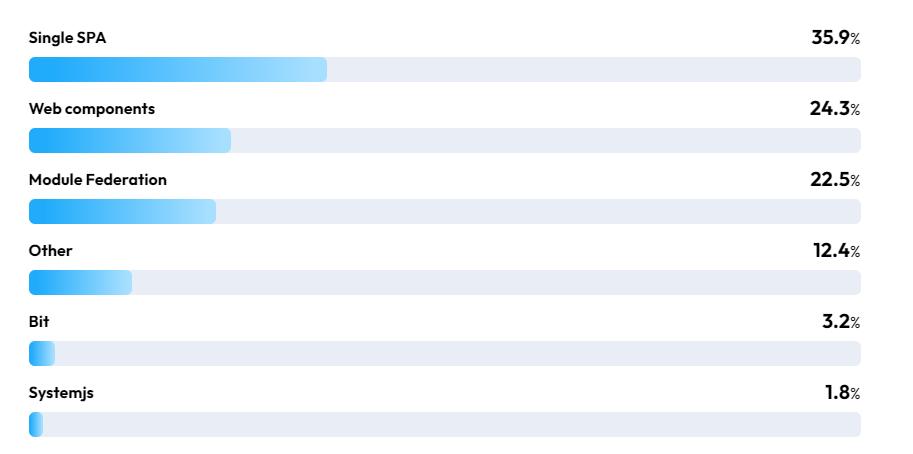
\includegraphics[width=\textwidth]{frontend_implementations_by_percent.png}
	\caption[Wykres procentowy popularności rozwiązań dla implementacji mikrofrontendów w 2022 roku]{Wykres procentowy popularności rozwiązań \\ dla implementacji mikrofrontendów w 2022 roku (źródło: \cite{tsh_2022})}
	\label{fig:tsh_frontend_implementations}
\end{figure}

Dla każdego z nich istnieje zestaw zastosowań biznesowych, dla których rozwiązanie nie będzie właściwe, ale będą istnieć też takie, dla których będą one właściwe. Każde z nich zostanie dokładniej omówione w poniższych podsekcjach.

\subsection{Konfiguracja serwera używająca routingu}
Konfigurowanie projektu, aby podawał do przeglądarki kod konkretnego mikrofrontendu w zależności od adresu URL można w prosty sposób wykonać poprzez odpowiednią konfigurację serwera. Taki sposób konfiguracji mkrofrontendów zalicza się do rozwiązań integrujących mikrofrontendy w czasie budowania projektu. To rozwiązanie jest wspierane przez najpopularniejsze oprogramowanie serwerowe takie jak IIS, Apache, NGINX. Konfiguracja serwera działa w bardzo prosty sposób - mapuje adresy URL na nazwy plików istniejących na serwerze oraz w zależności od tego, jaki aktualnie jest adres URL, przypisuje do zmiennej odpowiedni plik HTML. Odnosząc się do przykładu na listingu \cref{lst:nginx_microfrontends} (przykład pochodzi z \cite{fowler_2019}), taką zmienną jest \lstinline{$PAGE} z linii nr 8.

\lstinputlisting[style=htmlcssjs, label=lst:nginx_microfrontends, caption=Przykładowa implementacja mikrofrontendu wspomaganego przez NGINX]{listings/nginx_microfrontends.html}

\subsection{Elementy <iframe>}
Najprostszym rozwiązaniem, obecnym już od dawna w standardzie języka znaczników HTML, jest element \lstinline{<iframe>}. Zgodnie z teorią, takie rozwiązanie spełnia założenia mikrofrontendów. Elementy \lstinline{<iframe>} wygodny sposób izolują poszczególne mikrofrontendy od siebie, nie pozwalają na nadpisanie się selektorów CSS oraz ewentualnych zmiennych globalnych w skrpytach JavaScript. Dzieje się tak ze względu na to, że elementy \lstinline{<iframe>} posiadają swój osobny zakres dla styli CSS i kodu JavaScript. Mimo to mają one też kilka wad. Po pierwsze, pełna izolacja kontekstu w elemencie \lstinline{<iframe>} powoduje, że treść tego elementu strony nie będzie reagowała na zmiany w~routingu. Ponadto, operowanie na historii przeglądania, adresie URL jest znacznie utrudnione. Taki koncept sprawia też trudności w przypadku, gdy znaczenie ma responsywność strony. Przykładowa implementacja, pochodząca z \cite{fowler_2019} znajduje się na listingu \cref{lst:iframe_microfrontends}

\lstinputlisting[style=htmlcssjs, label=lst:iframe_microfrontends, caption=Przykładowa implementacja mikrofrontendu za pomocą \lstinline{<iframe>}]{listings/iframe_microfrontends.html}

\subsection{Przechowywanie mikrofrontendów w skryptach JavaScript}
Idea ładowania mikrofrontendów przez podpinanie skryptów JavaScript jest bardzo prosta. Zgodnie z przykładem implementacji podanym na listingu \cref{lst:js_microfrontends} (przykład pochodzi z \cite{fowler_2019}), na początku sekcji \lstinline{<body>} podpiete są trzy skrypty reprezentujące trzy mikrofrontendy. Obecny jest także element \lstinline{<div id="micro-frontend-root">}, do którego będą ładowane mikrofrontendy. W skrypcie podanym niżej znajduje się przyporządkowanie tras w routingu do mikrofrontendów o odpowiednich nazwach oraz referencja na element \lstinline{<div id="micro-frontend-root">}.

\lstinputlisting[style=htmlcssjs, label=lst:js_microfrontends, caption=Przykładowa implementacja mikrofrontendu za pomocą JavaScript]{listings/microfrontends.html}

\subsection{Dynamiczne ładowanie modułów poprzez menedżer pakietów}
Istnieje również grupa rozwiązań oparta na dynamicznym ładowaniu modułów. Do grupy rozwiązań tego typu należą wspomniane na wykresie procentowym z  \cref{fig:tsh_frontend_implementations}, Module Federation, Bit oraz Systemjs. Pierwsze z rozwiązań, Module Federation, jest wtyczką do transpilatora Webpack. Wszystkie trzy, pomimo pewnych niewielkich różnic w~zakresie składni poleceń, instalacji i procesu konfiguracji, działają bardzo podobnie.

\subsection{Single SPA}
Single SPA jest frameworkiem, za pomocą którego można zrealizować koncepcję mikrofrontendów. Ten framework czerpie swój sposób działania z rozwiązań opartych na dynamicznym ładowaniu modułów. Jednocześnie pod skórą, ten framework stosuje wspomniany wcześniej Systemjs do samego przygotowania modułów, które są później dynaminicznie ładowane do treści strony. Istnieje też więc możliwość używania Single SPA z~każdym innym popularnym frameworkiem stosowanym przez programistów frontendu. Innowacją, którą proponuje Single SPA są predefiniowane konfiguracje, które automatyzują tworzenie mikrofrontedów. Do celów automatyzacji ustawiania infrastruktury mikrofrontendów twórcy udostępniają narzędzie CLI o nazwie \textit{create-single-spa}. Single SPA narzuca też sam z siebie określony podział konkrentych mikrofrontendów ze względu na zastosowania. Składnikami tego podziału są:

\begin{itemize}
	\item \textit{root-config} - mikrofrontend mający zastosowanie głównie przy agregacji innych mikrofrontendów,
	\item \textit{application} - domyślny typ mikrofrontendu bez specjalnych zadań projektowych,
	\item \textit{parcel} - reużywalny komponent, który jest niezależny w konstrukcji od frameworków używanych w projekcie; w przypadku użycia tylko jednego frameworka w całym projekcie, twórcy rekomendują \cite{singlespa-parcels} poleganie na systemie komponentyzacji tego frameworka.
\end{itemize}

Oprócz wymienionych możliwości, framework Single SPA udostępnia swój interfejs do testów jednostkowych i testów E2E oraz wspiera renderowanie kodu strony po stronie serwera. Dokumentacja frameworka Single SPA zawiera bardzo dokładne instrukcje postawienia środowiska oraz wdrożenia produkcyjnego pod każdy z popularnych frameworków, co znacząco obniża próg wejścia w samą koncepcję mikrofrontendów.

\chapter{Funkcjonalność badanej aplikacji}
Na potrzeby porównania obu architektur stworzona została aplikacja do zarządzania finansami osobistymi o roboczej nazwie Midas. W założeniu odbiorcami aplikacji mają być pojedyncze osoby lub gospodarstwa domowe, które chcą zadbać o kontrolę nad swoim budżetem domowym. Głównymi funkcjonalnościami aplikacji są:

\begin{itemize}
	\item możliwość wykonywania operacji CRUD w zakresie informacji o wydatkach i~przychodach poszczególnych użytkowników,
	\item system autoryzacji i uwierzytelniania spełniający aktualne normy w zakresie bezpieczeństwa aplikacji sieciowych,
	\item system uprawnień w obrębie rodziny (przykładowo użytkownik o roli rodzica może edytować transakcje na kontach dzieci, a dzieci nie mogą podglądać transakcji rodziców),
	\item przechowywanie paragonów i faktur w wersji elektronicznej i możliwość przypisania ich do konkretnej transakcji.
\end{itemize}

Podany zestaw funkcjonalności umożliwi wydzielenie kilku mikroserwisów, co zapewni wystarczającą bazę do symulowania połączeń między serwisami. Wykonanie jej w~architekturze ściśle mikroserwisowej pozwoli jednocześnie dobudować do tych mikroserwisów poszczególne mikrofrontendy tak, aby stanowiły one razem pełnoprawne aplikacje komunikujące się między sobą. Z drugiej strony pozwoli to też dobudować monolityczny frontend, który będzie komunikował się ze wszystkimi serwisami. Dzięki takiemu posunięciu, dla obu badanych projektów - monolitycznego oraz mikrofrotendowego, zapewnione będą jednolite warunki w zakresie komunikacji z~backendem, co będzie stanowiło bazę do porównania obu koncepcji architektonicznych w~zakresie wydajności i dostępności.

\chapter{Opis backendu projektu}
\section{Dobór technologii do projektu}
Do zrealizowania tej części projektu został wykorzystany język C\# oraz środowisko .NET. Użyto środowiska .NET w wersji 6.0, która jest jednocześnie najnowszą dostępną wersją LTS (\textit{Long Term Support}). Wspomniane technologie są dobrym wyborem do realizacji mikroserwisów ze względu na:

\begin{itemize}
	\item użycie paradygmatu programowania obiektowego i będący jego częścią polimorfizm, który sprzyja replikacji pojedynczego wzorca mikroserwisu,
	\item będący częścią środowiska .NET framework ASP.NET realizujący architekturę REST przy niewielkim narzucie w ilości kodu,
	\item istnienie wielu gotowych klas i modeli realizujących podstawowe funkcje sieciowe, takie jak autoryzacja i autentykacja, komunikacja z bazą za pomocą Entity Framework,
	\item generator NSwag służący do generowania klas w językach C\# oraz TypeScript reprezentujących metody kontrolerów poszczególnych mikroserwisów wykonanych w ASP.NET.
\end{itemize}

Środowiska mikroserwisowe są de facto oddzielnymi serwisami działającymi jednocześnie i pobierającymi dostępne zasoby. Do celów testów lokalnych na komputerze programisty zachodzi więc potrzeba zastosowania rozwiązania, które zminimalizuje użycie zasobów komputera tak, aby jednocześnie zachować wierność odwzorowania środowiska z~wieloma serwerami. W celu osiągnięcia takiego efektu, zostało użyte oprogramowanie Docker służące do konteneryzacji środowisk. Za jego pomocą, używając specjalnych plików nazywanych obrazami, można tworzyć kontenery, którym Docker przydziela zasoby w czasie rzeczywistym tak, aby zoptymalizować ich użycie.
Razem z~narzędziem Docker, użyto też narzędzia Docker Compose \cite{dockercompose}, które umożliwia uruchomienie wielu kontenerów Dockera za pomocą pojedynczego skryptu.

Opisane technologie mogą też być używane w połączeniu z~oprogramowaniem Docker. Producent środowiska .NET, Microsoft udostępnił w serwisie Docker Hub obraz środowiska .NET z ustawionym frameworkiem ASP.NET i bazą SQL Server. Pozwala to na skorzystanie z gotowego środowiska, które jest konfigurowalne za pomocą pliku Dockerfile.

\section{Szablony projektów}
W celu zapewnienia skalowalności oraz łatwego tworzenia nowych serwisów, na potrzeby projektu opracowano dwa szablony projektu - zawierający wstępną autentykację użytkownika poprzez sprawdzanie zawartości nagłówka HTTP oraz taki, który jej nie zawiera.

Najważniejszą cechą tych szablonów jest możliwość szybkiego ustawienia nowego rozwiązania Visual Studio zawierającego ustawienia dla testów jednostkowych i~integracyjnych aplikacji, ustawienia plików \textit{Dockerfile} i \textit{docker-compose.yml} oraz ściśle określonego rozłożenia projektów w rozwiązaniu. Zapewnia to spójność kodu w zakresie całej aplikacji. W przypadku, gdyby nad kodem pojedynczego serwisu pracowało kilku programistów, mają oni ściśle narzuconą przez szablon strukturę kodu i podstawowa jego struktura zostanie zachowana. To z kolei powoduje, że wynikowo mimo tego, że nad poszczególnymi serwisami pracują różne osoby, ich struktura jest w dużym stopniu podobna. Ma to wiele zalet w zakresie zarządzania projektami, przykładowo:

\begin{itemize}
	\item pozwala na szybszą aklimatyzację programistów przenoszonych między projektami, bądź takich, których rola w zespole pomaga na wsparciu istniejących projektów,
	\item przyspiesza czas tworzenia nowych funkcjonalności oprogramowania,
	\item czas poświęcany na odtwórcze powtarzanie realizacji wzorca można poświęcić na ważniejsze czynności, takie jak redukcja długu technologicznego, zwiększanie pokrycia testami, itd.
\end{itemize}

\section{Podział backendu na serwisy}
Logika backendowa aplikacji została podzielona według funkcjonalności na serwisy opisane w poniższych podsekcjach.

\subsection{Hosting plików - File Storage Service}
Serwis z hostingiem plików odpowiada za przechowywanie wszystkich plików przekazanych aplikacji przez użytkownika. Są to między innymi zdjęcia profilowe użytkowników oraz pliki z dowodami wykonania transakcji przypisanych do konkretnych transakcji w ramach logiki domenowej. Serwis hostingu plików pozwala też na pobranie samego pliku o znanym identyfikatorze GUID oraz pobranie informacji o umieszczeniu pliku oraz konkretnych pobrań pliku.

\subsection{Autoryzacja - Authorization Service}
Serwis odpowiada za autoryzację użytkowników oraz operacje związane z~użytkownikami, które wymagają zachowania ostrożności pod kątem bezpieczeństwa aplikacji - tworzenie konta, logowanie do konta w aplikacji Midas, zmiana hasła. W tym serwisie przy logowaniu powstaje token JWT, który zapisany w ciasteczkach krąży po innych serwisach przekazywany przez nagłówek \textit{Authorization} w zapytaniu HTTP.

\subsection{Zarządzanie użytkownikami - User Service}
Serwis odpowiada za przechowywanie oraz umożliwienie dostępu do informacji o~użytkownikach. Obsługuje on też logikę związaną z kontami użytkowników, które nie wymagają zachowania szczególnej ostrożności w zakresie bezpieczeństwa aplikacji. Przykładem takiej operacji może być zmiana zdjęcia profilowego użytkownika.

\subsection{Zarządzanie rodzinami - Family Service}
Serwis odpowiada za przypisanie użytkowników do rodzin, których są członkami. Odpowiada też częściowo za uwierzytelnianie użytkownika - z tego serwisu pochodzą dane na temat tego, czy dany użytkownik ma wystarczające uprawnienia do edytowania danych dla swojej rodziny (ze względu na rolę przypisaną w systemie).

\subsection{Logika domenowa - Transaction Service}
Serwis ma za zadanie realizację operacji CRUD na transakcjach finansowych. Takimi operacjami może być wpisanie nowego wydatku do listy, usunięcie go z listy, pobranie listy wydatków w zależności do konkretnych parametrów (np. kategoria, czas, osoba z rodziny), dodanie pliku z dowodem wykonania transakcji.

\chapter{Opis badanych frontendów}
\section{Dobór technologii do projektów}
Do realizacji mikrofrontendów użyto biblioteki \textit{Single SPA}. Wspiera ona wszystkie najpopularniejsze frameworki do tworzenia aplikacji frontendowych. W badanych projektach użyto frameworka Angular ze względu na to, że najlepiej nadaje się do tworzenia dużych skalowalnych aplikacji. Ta cecha pozwoli utrzymać w ryzach rozbudowaną strukturę monolitycznej wersji projektu. W celu zapewnienia jak najmniejszych różnic technologicznych w projektach o różnej architekturze, wersja mikrofrontendowa będzie również używać frameworka Angular.

Do komunikacji z serwisami backendowymi, dla obu projektów użyto klas serwisów wygenerowanych przez generator NSwag. Będzie to działało tak, jak w przypadku klas w~języku C\# generowanych na potrzeby komunikacji między serwisami backendowymi. Różnica będzie tu jedynie taka, że te klasy będą gotowymi klasami w języku TypeScript dostosowanymi do użycia we frameworku Angular.

Ze względu na to, że walory estetyczne nie są istotne w zakresie rozważań nad mikrofrontendami, użyto gotowej biblioteki z elementami wizualnymi o nazwie \textit{angular-material}.

  \section{Wersja mikrofrontendowa}
  Logika frontendu aplikacji została podzielona na następujące mikrofrontendy:

  \begin{itemize}
    \item kontener (Container Microfrontend) - jest mikrofrontendem, do którego są ładowane wszystkie inne mikrofrontendy; jego zadaniem jest rozmieszczenie mikrofrontendów na stronie internetowej oraz kontrola ich ładowania poprzez reagowanie na zmiany w~routingu
    \item nawigacja (Navigation Microfrontend) - jest odpowiedzialny za ubranie możliwości przełączania się pomiędzy mikrofrontendami w sposób przyjazny dla użytkownika
    \item hosting plików (File Storage Microfrontend) - jego głównym zadaniem jest komunikacja z backendową częścią hostingu plików wspomnianą w rozdziale 4.3.1
    \item autoryzacja (Authorization Microfrontend) - jego głównym zadaniem jest komunikacja z backendową częścią autoryzacji wspomnianą w~rozdziale 4.3.2.
    \item zarządzanie użytkownikami (User Microfrontend) - jego głównym zadaniem jest komunikacja z backendową częścią zarządzania użytkownikami wspomnianą w~rozdziale 4.3.3.
    \item zarządzanie rodzinami (Family Microfrontend) - jego głównym zadaniem jest komunikacja z backendową częścią zarządzania rodzinami wspomnianą w~rozdziale 4.3.4.
    \item logika domenowa (Transaction Microfrontend) - jego głównym zadaniem jest komunikacja z backendową częścią zarządzania transakcjami wspomnianą w~rozdziale 4.3.5.
  \end{itemize}

  \subsection{Realizacja komunikacji między mikrofrontendami}
  W trakcie realizacji mikrofrontendowej wersji aplikacji wystąpiły dwie sytuacje, w~których nie było innego wyjścia niż zastosować komunikację bezpośrednio między mikrofrontendami.
  Pierwszą z nich jest fakt, że narzędzie Swagger błędnie serializalizuje obiekty odzwierciedlające pliki, gdy wykonuje serializację tego samego obiektu więcej niż jeden raz. Dlatego więc zamieszczanie plików było możliwe tylko bezpośrednio przez \textit{File Storage Service}, a to z kolei według założeń mikrofrontendów jest możliwe wyłącznie przez odpowiadający mu mikrofrontend - \textit{File Storage Microfrontend}. W tej sytuacji wystapiła potrzeba pobrania informacji dla \textit{Transaction Microfrontend} bezpośrednio z \textit{File Storage Microfrontend}. Dzięki temu zabiegowi można umieścić plik w hostingu plików za pomocą \textit{File Storage Microfrontend} i~przesłanie identyfikatora GUID pliku do \textit{Transaction Microfrontend}.

  Do tego celu zastosowano komunikację poprzez nasłuchiwanie zdarzeń. Wybór tej metody nastąpił ze względu na to, że komunikacja między tymi dwoma mikrofrontendami następowała tylko i wyłącznie we wspomnianej sytuacji. Generowanie paczki przez menedżer pakietów oraz użycie narzędzi do zarządzania stanem były zbyt skomplikowanymi rozwiązaniami na tak prosty przypadek. Zastosowanie \textit{Local Storage} lub ciasteczek powodowały w tym wypadku koniecnzość dodatkowych metod w komponentach służących do reagowania na zmiany w tych magazynach danych. Wybór padł więc na posłużenie się zdarzeniami w tym celu. Do implementacji tej funkcjonalności użyto trzech zdarzeń:

  \begin{itemize}
    \item \textit{file-upload} - do przekazania identyfikatora GUID pliku między serwisami
    \item \textit{reveal-upload} - do pokazania użytkownikowi elementów interfejsu realizujących przekazanie pliku
    \item \textit{hide-upload} - do schowania przed użytkownikiem elementów interfejsu realizujących przekazanie pliku
  \end{itemize}

  Implementacja tej funkcjonalności została przedstawiona na listingach \cref{lst:mf_communication_files} i \cref{lst:mf_communication_transactions}

  \lstinputlisting[style=es6, label=lst:mf_communication_files, caption=Implementacja komunikacji między mikrofrontendami po stronie \textit{Transaction Microfrontend}]{listings/mf_communiaction_file.ts}

  \vfill

  \lstinputlisting[style=es6, label=lst:mf_communication_transactions, caption=Implementacja komunikacji między mikrofrontendami po stronie \textit{File Storage Microfrontend}]{listings/mf_communiaction_transactions.ts}

  Metody \lstinline{ngOnInit} oraz \lstinline{ngOnDestroy} są elementami interfejsu \lstinline{OnInit}, który jest częścią frameworka Angular. Pierwsza z nich jest wywoływania zaraz po inicjalizacji komponentu, a druga przy jego usuwaniu. Są one odpowiednimi miejscami do tworzenia i~usuwania zdarzeń w zależności od warunków zdefiniowanych w kodzie pokazującym i~chowającym komponent. Komunikację między serwisami udało się zrealizować w~niespełna 40 linii kodu wliczając w to odpowiednie formatowanie, klamry oraz znaki nowej linii między metodami. Jest to odpowiednio proste rozwiązanie do tak prostego problemu. Co więcej, rozwiązanie jest łatwo skalowalne. Przy implementowaniu nowego komponentu wykorzystujące te zdarzenia wystarczy zdefiniować nowe metody w klasie komponentu, które będą się wywoływać przy nasłuchiwaniu zdarzenia.

  Drugą ze wspomnianych sytuacji jest pobieranie pliku z \textit{File Storage Service}. Implementacja przekazywania pliku przez backend do innego mikrofrontendu niż \textit{File Storage Microfrontend} byłaby nieoptymalna. Po pierwsze, przekazywanie pliku przez kilka serwisów zwiększa czas realizacji żądania HTTP. Po drugie takie rozwiązanie jest mało skalowalne - lepiej jest umożliwić potencjalne pobranie pliku z każdego dostępnego mikrofrontendu. W tej sytuacji można zastosować przekazywanie danych przez adres URL. Jedyną daną potrzebną do pobrania pliku jest identyfikator GUID pliku, a adres URL można ustawić w przeglądarce domyślnie za pomocą każdego mikrofrontendu z każdego komponentu. Poza tym, do realizacji pobierania pliku nie jest potrzebny żaden interfejs graficzny, a jedynie metoda pobierająca identyfikator z adresu URL i metoda pobierająca dane z \textit{File Storage Service}. Implemetacja funkcjonalności została przedstawiona na listingu \cref{lst:mf_downloading_file}

  \lstinputlisting[style=es6, label=lst:mf_downloading_file, caption=Komponent realizujący pobieranie pliku przy użyciu danych z adresu URL , extendedchars=true,literate={±}{{$\pm$}}1 {§}{{\S}}1]{listings/mf_downloading_file.ts}

  W linii 13, pobierany jest parametr z adresu URL, który w module realizującym routing aplikacji nazwano \textit{guid}. Ten parametr jest następnie sprawdzany za pomocą metody \lstinline{checkIfGuidIsValid}, która sprawdza czy parametr został poprawnie podany do komponentu. Następnie pobierany jest plik z odpowedniego serwisu za pomocą metody \lstinline{sendDownloadRequest}, a potem ten plik jest pobierany z komponentu na dysk użytkownika za pośrednictwem przeglądarki w metodzie \lstinline{downloadFile}.

\chapter{Porównanie projektów frontendowych}
  W celu zapewnienia jak największej zgodności między oboma projektami, tam gdzie jest to możliwe, logika komponentów w obu projektach jest dokładnie taka sama. W innych przypadkach, dokonano możliwie jak najprostszych korekt, aby oba projekty się skompilowały. Ponad to, w pliku \textit{angular.json} w każdym z mikrofrontendów dopisano do konfiguracji Webpacka opcję \lstinline{"excludeAngularDependencies": true}, co pozwoliło na to, żeby nie importować zależności frameworka Angular za każdym zbudowaniem aplikacji. Zamiast tego, te pliki są ładowane z repozytoriów CDN, do których dane zapisano w \textit{Container Microfrontend} w folderze \lstinline{import_maps}.

  \section{Metryki kodu}
    \subsection{Ilość kodu}
    W celu sprawdzenia ilości kodu napisanego w obu projektach użyto paczki \textit{cloc} dostępnej w systemie Linux. Za jej pomocą można policzyć ile linii tekstu zawiera plik lub folder oraz przyporządkowuje je do jednej z trzech kategorii.

    \begin{itemize}
      \item \textit{blank} - pusta linia
      \item \textit{comment} - komentarz
      \item \textit{code} - linia kodu
    \end{itemize}

    Za pomocą tego narzędzia sprawdzono foldery \lstinline{src} wszystkich frontendów w obu projektach. Inne foldery zostały wyłączone ze sprawdzenia, gdyż zawierają one metadane projektów, pliki menadżera pakietów lub też dane generowanie automatyczne. One wszystkie nie są narzutem kodu bezpośrednio wygenerowanym przez programistę - wzięcie ich pod uwagę mogłoby wypaczyć wyniki pod względem wpływu kodu na powstanie projektu. Wyniki sprawdzenia zostały pokazane w \cref{table:cloc}

    \begin{table}[h]
      \centering
      \caption{Wyniki sprawdzenia ilości kodu za pomocą \textit{cloc}}
      \begin{tabular}{|l||r|r|r|r|r|}
      \hline
      \textbf{Mikrofrontend} & \multicolumn{1}{l|}{\textbf{Pliki}} & \multicolumn{1}{l|}{\textbf{Puste linie}} & \multicolumn{1}{l|}{\textbf{Komentarze}} & \multicolumn{1}{l|}{\textbf{Linie kodu}} & \multicolumn{1}{l|}{\textbf{Suma linii}} \\ \hline
      \textit{Authorization} & 41 & 196 & 98 & 1124 & 1459 \\ \hline
      \textit{Users} & 41 & 236 & 132 & 1511 & 1920 \\ \hline
      \textit{Transactions} & 47 & 375 & 216 & 2369 & 3007 \\ \hline
      \textit{File Storage} & 34 & 201 & 162 & 1234 & 1631 \\ \hline
      \textit{Family} & 40 & 279 & 144 & 1731 & 2194 \\ \hline
      \textit{Navigation} & 29 & 87 & 70 & 438 & 624 \\ \hline
      \textit{Container} & 4 & 17 & 24 & 121 & 166 \\ \hline
      \textbf{SUMA}& 236 & 1391 & 846 & 8528 & \textbf{11001} \\ \hline\hline
      \textit{Monolityczny frontend} & 113 & 1053 & 407 & 7023 & \textbf{8596} \\ \hline
      \end{tabular}
      \label{table:cloc}
    \end{table}

    Wyniki pokazują, że w porównaniu do frontendu monolitycznego, identyczne funkcjonalności zajmują ponad dwa razy więcej plików w projekcie mikrofrontendowym. Ponadto projekt mikrofrontendowy zawiera 21,43\% linii więcej samego kodu, a~w~ogólności 27,98\% więcej linii tekstu.
  
    \subsection{Paczki z plikami wynikowymi}
    Aplikacje zbudowano za pomocą komendy \lstinline{ng build} w aplikacjach z frameworkiem Angular oraz komendy \lstinline{webpack --mode=production} dla aplikacji kontenera. Czasy budowania aplikacji oraz rozmiary paczek przedstawia \cref{table:build_times}.

    \begin{table}[h]
      \centering
      \caption{Czasy budowania aplikacji oraz rozmiary paczek wynikowych}
      \begin{tabular}{|l||r|r|}
      \hline
      \textbf{Mikrofrontend} & \multicolumn{1}{l|}{\textbf{Czas {[}s{]}}} & \multicolumn{1}{l|}{\textbf{Rozmiar paczki {[}kB{]}}} \\ \hline
      \textit{Authorization} & 12,53 & 341,00 \\ \hline
      \textit{Users} & 13,13 & 367,98 \\ \hline
      \textit{Transactions} & 14,41 & 486,23 \\ \hline
      \textit{FileStorage} & 11,68 & 193,40 \\ \hline
      \textit{Family} & 13,09 & 369,46 \\ \hline
      \textit{Navigation} & 9,68 & 139,85 \\ \hline
      \textit{Container} & 2,47 & 20,40 \\ \hline
       \textbf{SUMA} & \textbf{76,99} & \textbf{1918,32} \\ \hline\hline
       \textit{Monolityczny frontend} & \textbf{27,12} & \textbf{938,07} \\ \hline
      \end{tabular}
      \label{table:build_times}
    \end{table}

    Niestety \lstinline{angular-cli}, które jest częścią frameworka Angular, nie posiada narzędzi, które pozwalałyby budować kilka aplikacji na raz. Jednocześnie komenda budująca paczkę wynikową jest zależna od ścieżki w której użytkownik się znajduje. Utrudnia to znacząco stworzenie skryptu automatyzującego, który wykonywałby komendy jednocześnie. Można więc przyjąć, że w przeciętnym projekcie informatycznym programista w najbardziej pesymistycznej sytuacji potencjalnie wykonuje te komendy jedna po drugiej, bądź używa skryptu, który nie zapewnia wykonywania się kilku komend jednocześnie. Jednak w~przeciętnych warunkach taka sytuacja nie nastąpi - budowanie dwóch aplikacji w~założeniach mają wykonywać dwa odrębne zespoły. Taki pojedynczy zespół, w~najgorszym wypadku (dla \textit{Transactions Microfrontend}) budowałby swoją część aplikacji o połowę szybciej niż cały frontend monolityczny.

    Wyniki z \cref{table:build_times} pokazują, że łączny czas budowania całego projektu jest 183\% większy dla projektu mikrofrontendowego niż dla projektu z monolitycznym frontendem. Rozmiar paczki wynikowej w projekcie mikrofrontendowym jest o 104\% większy niż dla projektu monolitycznego. Należy zaznaczyć, że nie wynika z tego jeszcze, że przeglądarka użytkownika będzie musiała jednorazowo pobrać więcej danych, aby aplikacja poprawnie działała.

    \subsection{Czas ładowania aplikacji do przeglądarki internetowej}
    W celu wykonania testów czasu ładowania aplikacji do przeglądarki przeprowadzono test ładowania witryny na niektórych widokach z wyczyszczoną uprzednio pamięcią podręczną. Ten test oraz kolejne wykonano na 64-bitowej przeglądarce Chrome w wersji 108, na systemie operacyjnym Linux Mint. Wyniki są pokazane w \cref{table:runtimes_without_cache}.

    \begin{table}[h]
      \centering
      \caption{Czasy ładowania aplikacji przy wyczyszczonej pamięci podręcznej przeglądarki}
      \begin{tabular}{l|rrr|}
      \cline{2-4}
       & \multicolumn{3}{c|}{\textbf{Czas załadowania widoku {[}s{]}}} \\ \hline
      \multicolumn{1}{|l|}{\textbf{Projekt}} & \multicolumn{1}{l|}{\textbf{Transakcje}} & \multicolumn{1}{l|}{\textbf{Profil użytkownika}} & \multicolumn{1}{l|}{\textbf{Lista rodzin}} \\ \hline
      \multicolumn{1}{|l|}{\textit{mikrofrontendowy}} & \multicolumn{1}{r|}{1,770} & \multicolumn{1}{r|}{1,460} & 1,770 \\ \hline
      \multicolumn{1}{|l|}{\textit{monolityczny}} & \multicolumn{1}{r|}{0,386} & \multicolumn{1}{r|}{0,322} & 0,327 \\ \hline
      \end{tabular}
      \label{table:runtimes_without_cache}
    \end{table}

    Z pustą pamięcią podręczną widok transakcji oraz widok profilu użytkownika w~projekcie mikrofrontendowym ładują się do przeglądarki ponad 4 razy wolniej, a widok listy rodzin ponad 5 razy wolniej. Jest to efekt tego, że przy pustej pamięci podręcznej, skrypt pobiera biblioteki przy użyciu podanego wcześniej pliku z odnośnikami do zewnętrznych bibliotek.

    Wykonano też po 10 uruchomień aplikacji w obu omawianych projektach i zmierzono czasy ładowania tych samych widoków, co w poprzednim teście. Następnie wyznaczono dla obu projektów średnią ze wszystkich pomiarów. W tym przypadku jednak, skorzystano z~tego, że zewnętrzne biblioteki są załadaowane do pamięci podręcznej przeglądarki. Wyniki pomiarów przedstawia \cref{table:runtimes_with_cache}.
    
    \vfill

    \begin{table}[]
      \centering
      \caption{Czasy ładowania aplikacji przy bibliotekach w pamięci podręcznej przeglądarki}
      \begin{tabular}{ll|rrr|}
      \cline{3-5}
       &  & \multicolumn{3}{c|}{\textbf{Czas załadowania widoku {[}s{]}}} \\ \hline
      \multicolumn{1}{|l|}{\textbf{Nr}} & \textbf{Projekt} & \multicolumn{1}{l|}{\textbf{Transakcje}} & \multicolumn{1}{l|}{\textbf{Profil użytkownika}} & \multicolumn{1}{l|}{\textbf{Lista rodzin}} \\ \hline
      \multicolumn{1}{|r|}{\textbf{1}} & \textit{mikrofrontendowy} & \multicolumn{1}{r|}{0,402} & \multicolumn{1}{r|}{0,407} & 0,445 \\ \hline
      \multicolumn{1}{|l|}{\textbf{}} & \textit{monolityczny} & \multicolumn{1}{r|}{0,181} & \multicolumn{1}{r|}{0,136} & 0,211 \\ \hline
      \multicolumn{1}{|r|}{\textbf{2}} & \textit{mikrofrontendowy} & \multicolumn{1}{r|}{0,402} & \multicolumn{1}{r|}{0,351} & 0,441 \\ \hline
      \multicolumn{1}{|l|}{\textbf{}} & \textit{monolityczny} & \multicolumn{1}{r|}{0,214} & \multicolumn{1}{r|}{0,183} & 0,267 \\ \hline
      \multicolumn{1}{|r|}{\textbf{3}} & \textit{mikrofrontendowy} & \multicolumn{1}{r|}{0,434} & \multicolumn{1}{r|}{0,389} & 0,479 \\ \hline
      \multicolumn{1}{|l|}{\textbf{}} & \textit{monolityczny} & \multicolumn{1}{r|}{0,145} & \multicolumn{1}{r|}{0,138} & 0,230 \\ \hline
      \multicolumn{1}{|r|}{\textbf{4}} & \textit{mikrofrontendowy} & \multicolumn{1}{r|}{0,422} & \multicolumn{1}{r|}{0,437} & 0,375 \\ \hline
      \multicolumn{1}{|l|}{\textbf{}} & \textit{monolityczny} & \multicolumn{1}{r|}{0,214} & \multicolumn{1}{r|}{0,136} & 0,183 \\ \hline
      \multicolumn{1}{|r|}{\textbf{5}} & \textit{mikrofrontendowy} & \multicolumn{1}{r|}{0,405} & \multicolumn{1}{r|}{0,501} & 0,411 \\ \hline
      \multicolumn{1}{|l|}{\textbf{}} & \textit{monolityczny} & \multicolumn{1}{r|}{0,229} & \multicolumn{1}{r|}{0,169} & 0,163 \\ \hline
      \multicolumn{1}{|r|}{\textbf{6}} & \textit{mikrofrontendowy} & \multicolumn{1}{r|}{0,416} & \multicolumn{1}{r|}{0,369} & 0,351 \\ \hline
      \multicolumn{1}{|l|}{\textbf{}} & \textit{monolityczny} & \multicolumn{1}{r|}{0,164} & \multicolumn{1}{r|}{0,150} & 0,223 \\ \hline
      \multicolumn{1}{|r|}{\textbf{7}} & \textit{mikrofrontendowy} & \multicolumn{1}{r|}{0,390} & \multicolumn{1}{r|}{0,427} & 0,402 \\ \hline
      \multicolumn{1}{|l|}{\textbf{}} & \textit{monolityczny} & \multicolumn{1}{r|}{0,188} & \multicolumn{1}{r|}{0,189} & 0,156 \\ \hline
      \multicolumn{1}{|r|}{\textbf{8}} & \textit{mikrofrontendowy} & \multicolumn{1}{r|}{0,481} & \multicolumn{1}{r|}{0,377} & 0,379 \\ \hline
      \multicolumn{1}{|l|}{\textbf{}} & \textit{monolityczny} & \multicolumn{1}{r|}{0,192} & \multicolumn{1}{r|}{0,127} & 0,144 \\ \hline
      \multicolumn{1}{|r|}{\textbf{9}} & \textit{mikrofrontendowy} & \multicolumn{1}{r|}{0,437} & \multicolumn{1}{r|}{0,371} & 0,471 \\ \hline
      \multicolumn{1}{|l|}{\textbf{}} & \textit{monolityczny} & \multicolumn{1}{r|}{0,161} & \multicolumn{1}{r|}{0,134} & 0,180 \\ \hline
      \multicolumn{1}{|r|}{\textbf{10}} & \textit{mikrofrontendowy} & \multicolumn{1}{r|}{0,485} & \multicolumn{1}{r|}{0,366} & 0,403 \\ \hline
      \multicolumn{1}{|l|}{\textbf{}} & \textit{monolityczny} & \multicolumn{1}{r|}{0,210} & \multicolumn{1}{r|}{0,169} & 0,142 \\ \hline\hline
      \multicolumn{1}{|l|}{\textbf{ŚREDNIA}} & \textit{mikrofrontendowy} & \multicolumn{1}{r|}{0,427} & \multicolumn{1}{r|}{0,400} & 0,416 \\ \hline
      \multicolumn{1}{l|}{} & \textit{monolityczny} & \multicolumn{1}{r|}{0,190} & \multicolumn{1}{r|}{0,153} & 0,190 \\ \cline{2-5} 
      \end{tabular}
      \label{table:runtimes_with_cache}
    \end{table}

    Wyniki pokazują, że średnio aplikacja ładuje się wolniej w projekcie mikrofrontendowym niż w projekcie monolitycznym o następujące wartości w punktach procentowych:

    \begin{itemize}
      \item widok transakcji - 125\%
      \item widok profilu użytkownika - 161\%
      \item widok listy rodzin - 118\%
    \end{itemize}

    Oba testy pokazują, że pod względem ładowania aplikacji do przeglądarki, lepsze osiągi prezentuje projekt monolityczny. Nie pomaga w tym zakresie wcześniej zastosowana i~sugerowana w dokumentacji \cite{singlespa} optymalizacja pod względem ładowania dla wszystkich mikrofrontendów z zewnętrznych źródeł.

  \section{Rozkład architektoniczny projektu}
  Schematy projektów obu aplikacji znajdują się na poniższych rysunkach. Na \cref{fig:monolith_fe_diagram}, zielone prostokąty odzwierciedlają mikrofrontendy realizujące konkretne funkcjonalności, natomiast kontener oznaczono kolorem szarym. Na \cref{fig:microservices_fe_diagram}, cały frontend monolityczny jest oznaczony kolorem szarym.

  \begin{figure}[h!]
    \centering
    \captionsetup{justification=centering}
    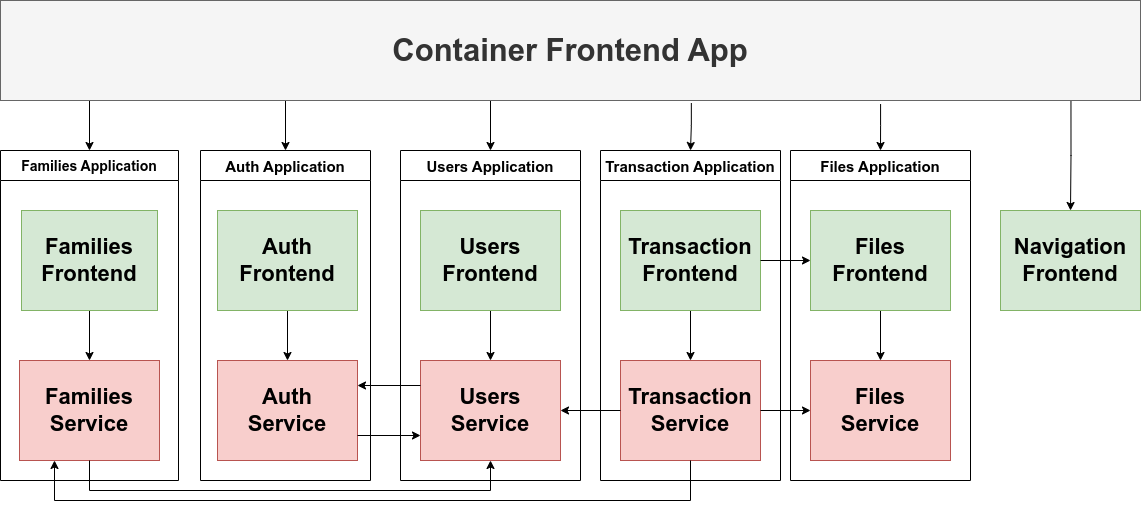
\includegraphics[width=\textwidth]{microfrontend-app-architecture.png}
    \caption{Schemat projektu aplikacji z mikrofrontendami z podziałem na moduły}
    \label{fig:monolith_fe_diagram}
  \end{figure}

  \pagebreak

  \begin{figure}[h]
    \centering
    \captionsetup{justification=centering}
    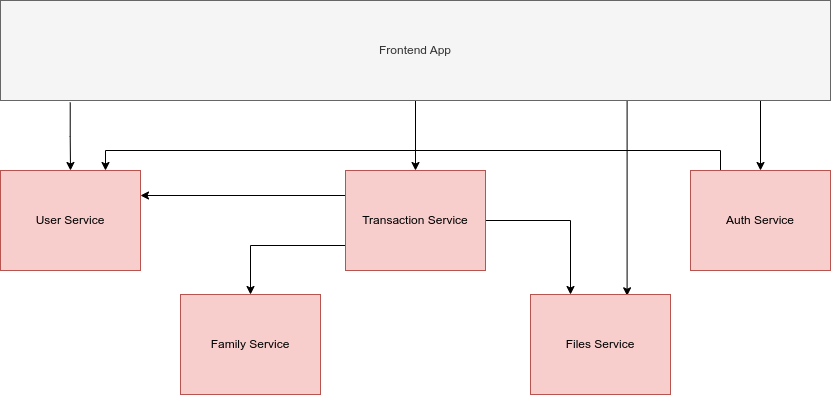
\includegraphics[width=\textwidth]{microservices-app-diagram.png}
    \caption{Schemat projektu aplikacji monolitycznej bez podziału na moduły}
    \label{fig:microservices_fe_diagram}
  \end{figure}

  W mikrofrontendowej wersji można wyodrębnić pięć osobnych aplikacji, nad którymi równolegle może pracować pięć osobnych zespołów. Jedynym zastrzeżeniem jest to, że 
  zespół pracujący nad \textit{File Storage Microfrontend} musiałby ukończyć swoje prace wcześniej niż zespół pracujący nad \textit{Transactions Microfrontend}.

  W wersji monolitycznej natomiast każdy podział aplikacji jest wciąż zamknięty technicznie w obrębie jednej aplikacji. W tak małej skali, jaką ma projekt, na którym oparte jest to porównanie, można przykładowo podzielić aplikację na moduły. W omawianym projekcie monolitycznym moduły zostały umieszczone w folderze \lstinline{/src/app/modules}. Schemat tego podziału został umieszczony na \cref{fig:monolith_fe_modules_diagram}.

  \begin{figure}[h]
    \centering
    \captionsetup{justification=centering}
    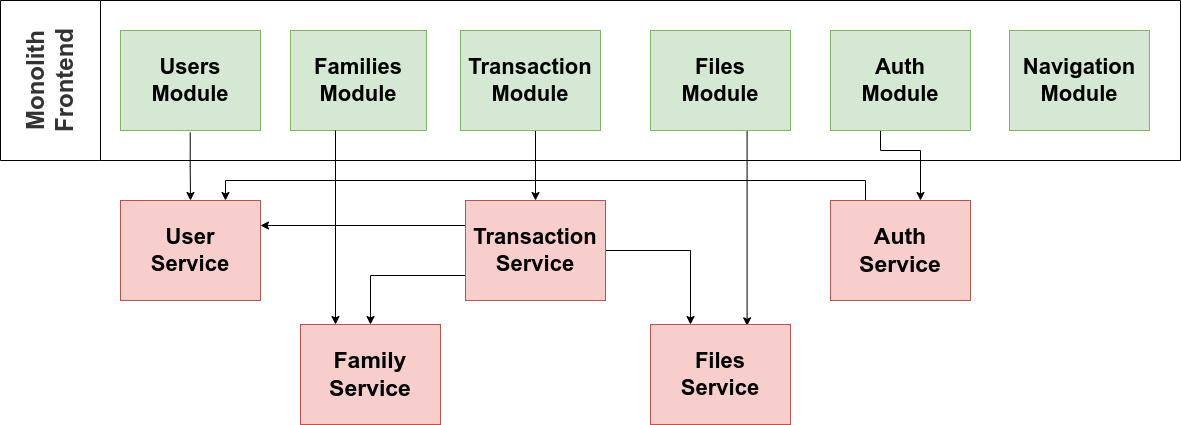
\includegraphics[width=\textwidth]{mfe-modules.png}
    \caption{Schemat projektu aplikacji monolitycznej z podziałem na moduły}
    \label{fig:monolith_fe_modules_diagram}
  \end{figure}

  Taki podział działa w niewielkiej skali. Jednak w przypadku, gdyby projekt miał 100 lub 1000 mikrofrontendów, czas budowania aplikacji wzrósłby do ogromnych wartości, a~oddzielne mikrofrontendowe aplikacje będą się budować dalej w czasie odpowiednim tylko dla ich zakresu domenowego. Dlatego więc podział na moduły jest w ogólności wyłącznie półśrodkiem.

  Dyskusja odnośnie podziału aplikacji ma duże znaczenie w kontekście skalowania aplikacji. Dodanie kolejnej warstwy do projektu aplikacji oznacza jedynie konieczność dodania referencji wyłącznie w jednej aplikacji. W przypadku projektu mikrofrontendowego oznacza to konieczność dodania referencji w każdym mikrofrontendzie, który miałby komunikować się z tą kolejną warstwą. Dlatego więc aplikacja monolityczna będzie się lepiej skalować wertykalnie.

  W przypadku skalowania horyzontalnego, odrobinę korzystniej wypada architektura mikrofrontendowa. Ilość referencji do dodania w warstwie, w której dochodzi do skalowania jest taka sama dla obu projektów. Programiści implementujący nowe funkcjonalności są jednak wciąż zależni od bazy kodu, którą zastali. Jednak w przypadku mikrofrontendów, zgodnie z ich założeniami, dodawanie nowych mikrofrontendów odbywa się niezależnie od reszty kodu aplikacji. Sprzyja to zdecydowanie skalowaniu horyzontalnemu aplikacji.

  \section{Infrastruktura i koszty}
  Infrastruktura potrzebna do uruchomienia pojedynczej aplikacji frontendowej nie jest skomplikowana. Istnieje wybór spośród wielu serwerów WWW, przykładowo:

  \begin{itemize}
    \item Apache
    \item Node.js
    \item Nginx
    \item IIS
  \end{itemize}

  Do każdego z tych serwerów, w Internecie istnieje wielu usługodawców oferujących usługi hostingu WWW. Rynek usług hostingu WWW rozwinął się na tyle, że udostępnienie witryny w internecie stało się bardzo proste.

  Sytuacja w przypadku mikrofrontendów daje większe pole do popisu specjalistom od infrastruktury sieciowej. Omawiany projekt mikrofrontendowy składa się już nie z jednej aplikacji, a z siedmiu osobnych aplikacji. W tak małej skali w jakiej jest przykładowy projekt, dałoby się skorzystać z tych samych rozwiązań, co dla frontendu monolitycznego. Wiele usługodawców \cite{ovh, az} oferuje swoim klientom nielimitowaną ilość stron WWW w~ramach jednej oferty. Dzięki temu, koszty wystawienia projektu mikrofrontendowego do Internetu są podobne, jak dla projektu monolitycznego. Dla obu omawianych projektów minimalny poniesiony koszt jest taki sam.
  
  Jednak przy dużej ilości mikrofrontendów, zarządzanie wieloma stronami wystawionymi do hostingu WWW może stać się kłopotliwe. W takiej sytuacji lepiej sprawdzają się inne rozwiązania, które pomagają w zarządzaniu wieloma aplikacjami jednocześnie. Przykładami takich rozwiązań mogą być \textit{Amazon Elastic Kubernetes Services (EKS)} i \textit{Azure Kubernetes Services (AKS)}. Oba rozwiązania wykorzystują narzędzie Kubernetes \cite{kubernetes} służące do automatyzacji i skalowania rozwiązań kontenerowych.

  Oba omawiane przykładowe projekty mikrofrontendowe posiadają wykonane konfiguracje do narzędzia Docker, które pozwalają na konteneryzację środowiska oraz uruchomienie w nim kodu aplikacji oraz budowania obrazów, które mogą być później wykorzystane przez Kubernetes. Na potrzeby lokalnego uruchomienia aplikacji został stworzony skrypt uruchamiający konfiguracje \textit{docker-compose} dla każdego serwisu i~mikrofrontendu w aplikacji. W razie potrzeby udostępnienia tego w Internecie istnieje możliwość szybkiego zmigrowania aplikacji do klastrów Kubernetes oferowanych przez dostępnych dostawców usług chmurowych. Koszty klastra Kubernetes w usłudze AKS \cite{aks_calc} w konfiguracji B2s z dwoma rdzeniami procesora, 4 GB pamięci RAM oraz 8 GB pamięci masowej na dysku HDD, wynosi 36,21 USD miesięcznie lub w przypadku trzyletniej rezerwacji - 13,61 USD miesięcznie. Warto przy tym pamiętać, że jest to najbardziej budżetowa wersja tej usługi - wszystkie dodatkowe udogodnienia wiążą się też z~dodatkowymi kosztami.

  \section{Testowanie kodu}
  Pomiędzy obiema wersjami projektu nie ma różnic w zakresie uruchamiania oraz tworzenia testów automatycznych. Głównym powodem takiego wyniku może być fakt, że we frameworku Angular, testy jednostkowe są wykonywane w odniesieniu do komponentu. Nie ma znaczenia to, w jakim środowisku został umieszczony komponent - można więc też wnioskować, że zmiana architektury projektu z monolitycznej na mikroserwisową nie wpływa na takie czynniki testowania takie jak:
  
  \begin{itemize}
    \item czas uruchomienia siatki testów automatycznych
    \item poziom ich skomplikowania
    \item ilość zależności potrzebnych do poprawnego odwzorowania logiki komponentu
  \end{itemize}

  Zgadza się to z wnioskami Micheala Geersa \cite{geers_2020}, jak i Martina Fowlera \cite{fowler_2019} w zakresie testów automatycznych na warstwie frontendu aplikacji.

  Jednakże, istnieją różnice w zakresie testowania manualnego obu wersji aplikacji. W~przypadku, gdy wystąpi błąd przy komunikacji z backendowym odpowiednikiem mikrofrontendu, będzie się różnił zakres kodu, w którym został popełniony błąd - na korzyść architektury mikrofrontendowej. W aplikacji mikrofrontendowej, analizując zrzut stosu aplikacji można się przede wszystkim dowiedzieć, z którego mikrofrontendu pochodzi dany błąd, co zawęża zakres poszukiwań przyczyny błędu.

  \section{Zależności między modułami i projektami}
  Do każdego mikrofrontendu użyto kilku zewnętrznych bibliotek, z czego duża z nich pokrywała się w większości mikrofrontedów. Przykładami takich często używanych zależności są pliki bibliotek: \textit{Single SPA}, \textit{Angular}, \textit{Angular Material}. Taka sytuacja powoduje, że użytkownik jest zmuszany do pobierania tych samych bibliotek więcej niż jeden raz. To powoduje, że do przeglądarki jest pobierane więcej danych niż jest to potrzebne. Część z tych problemów przy realizacji mikrofrontendowej wersji projektu udało się rozwiązać poprzez zadeklarowanie przy budowaniu aplikacji, żeby nie dodawać do paczki ze zbudowaną aplikacją tych bibliotek. Takie pliki będą pobierane raz przy pierwszym odwiedzeniu witryny z aplikacją. Odnośniki do takich bibliotek zostały zebrane w plikach typu JSON w folderze \lstinline{import_maps} aplikacji \textit{Container Microfrontend}. Listing \cref{lst:import_map} zawiera plik z odnośnikami do bibliotek, który posłużył do manualnych testów aplikacji.

  \lstinputlisting[style=es6, label=lst:import_map, caption=Obiekt zawierający odnośniki do bibliotek z zewnętrznych źródeł]{listings/import_map.json}

  Części zależności nie udało się wyłączyć z paczki wynikowej aplikacji. Mimo to, udało się uniknąć tego problemu dla największych i najbardziej istotnych bibliotek.

  \pagebreak

  \section{Możliwości w zakresie zarządzania projektami}
  Możliwość podziału aplikacji na wiele niezależnych od siebie bytów stanowi szansę na ograniczenie ilości węzłów komunikacyjnych między odrębnymi zespołami. Potencjalnymi skutkami tego rodzaju optymalizacji są:

  \begin{itemize}
    \item zmniejszenie ilości spotkań,
    \item zmniejszenie ilości osób, które są potrzebne do wprowadzenia ustaleń krytycznych dla projektu,
    \item wprowadzenie oddzielnych cykli planowania dla poszczególnych cykli produkcji aplikacji,
    \item możliwość pracy nad wieloma częściami aplikacji jednocześnie,
    \item zmniejszenie ilości wiedzy na temat projektu krytycznie potrzebnej dla nowej osoby w projekcie do skutecznego wdrożenia
  \end{itemize}  

  Jednak warto zauważyć, że ważny jest sam fakt zaprojektowania aplikacji w taki sposób, aby poszczególne części projektu były możliwie najbardziej niezależne od siebie nawzajem. Na rysunkach \cref{fig:microservices_fe_diagram} i \cref{fig:monolith_fe_modules_diagram} widać, że taki podział jest możliwy w przypadku obu omawianych projektów.

  Prawo Conwaya \cite{conway} mówi o tym, że "każda organizacja, wytwarza produkt, który jest odwzorowaniem jej struktury organizacyjnej". Oznacza to, że fakt wpływu struktury zarządzania firmy na projekt programistyczny, jest według tego prawa implikacją jednostronną. Można z tego wywnioskować, że niezależnie od tego, nawet projekt zrealizowany przy użyciu mikrofrontendów przy wadliwym zarządzaniu projektem nie uratuje zespołu projektowego od wszystkich czynników, które mają być w~założeniach optymalizowane przez mikrofrontendy.

  Wzrost ilości infrastruktury potrzebnej do utrzymania mikrofrontendów powoduje również zapotrzebowanie na większą ilość osób zajmujących się \textit{inżynierią DevOps}. Zależnie od potrzeb biznesowych, może się też okazać, że potrzebne są dodatkowe godziny spotkań w sprawie infrastruktury mikrofrontendowej, narzędzi potrzebnych do wdrożenia produkcyjnego i deweloperskiego aplikacji. Ten czynnik może spowodować, że mikrofrontendy, które w założeniu miały zoptymalizować komunikację w zespole projektowym, jedynie przeniosą zaoszczędzone w ten sposób godziny robocze na inny obszar projektu, bądź nawet wydłużą w czasie prace nad projektem.

\chapter{Podsumowanie}
Pod względem osiągów technicznych, na wszystkich zaprezentowanych polach lepiej prezentuje się projekt wykonany w architekturze monolitycznej. Zawartość aplikacji pojawia się szybciej na ekranie użytkownika w tym projekcie oraz przy procesie ładowania zawartości pobierana jest mniejsza ilość danych. Jest możliwe, że dla większej skali projektu, wyniki są inne.

Projekt monolityczny generuje również mniej plików oraz mniej linii kodu. Jednak pojedyncza aplikacja mikrofrontendowa buduje się szybciej niż cały projekt monolityczny. Powoduje to, że po dokonaniu zmiany w projekcie, szybsze będzie zbudowanie tego mikrofrontendu, który zawierał zmianę niż całego monolitu - zwiększa to potencjalnie komfort pracy nad projektem, a w dużej skali może zaowocować oszczędnością na czasie. Pod tym względem, mikrofrontendowy projekt oferuje więcej niż monolityczny.

Testowanie obu projektów niczym się nie różni. Jest to możliwe dzięki zastosowaniu paradygmatu programowania komponentowego do budowy pojedynczej aplikacji we frameworku \textit{Angular}. Możliwe są jedynie odstępstwa przy testach integracyjnych i E2E.

Struktura architektoniczna projektu mikrofrontendowego jest teoretycznie bardziej skomplikowana niż projektu monolitycznego. Jednak gdyby wziąć przy rozważaniu monolitu pod uwagę szczegółową budowę modułów, może się okazać, że struktura aplikacji jest podobna, jeśli nie identyczna jak mikrofrontendowa. Dlatego ważny jest sam fakt podzielenia aplikacji oraz rozwagi w procesie tworzenia aplikacji, a później jej utrzymywania i skalowania. W praktyce, projekt mikrofrontendowy ma lepsze możliwości skalowania horyzontalnego, a projekt monolityczny lepiej się skaluje wertykalnie ze względu na mniejszą ilość zależności. W tym zakresie, obie koncepcje architektoniczne mogą się nadawać do spełnienia konkretnych potrzeb biznesowych.

Skomplikowanie struktury projektu po stronie mikrofrontendów powoduje też wzrost liczby zależności, które są powtarzane w wielu mikrofrontendach. Pomimo zastosowania technik optymalizacyjnych, nie osiągnięto wydajności na poziomie projektu monolitycznego. Częściowo odpowiedzialny jest za to dodatkowy narzut w postaci dodatkowej (w stosunku do monolitu) biblioteki \textit{Single SPA}. Większa ilość zależności w~projekcie mikrofrontendowym jest zdecydowanie jego wadą.

W zakresie zarządzania projektami, dobrze zarządzany proces produkcji oprogramowania będzie prowadził do sukcesu zarówno przy zastosowaniu mikrofrontendów jak i przy zwykłym monolicie. Nie można zawierzyć powodzenia projektu jedynie zastosowanej architekturze oprogramowania. Dużo ważniejsza w tym zakresie jest struktura organizacyjna w zespole, który podejmuje się produkcji oprogramowania.

Podsumowując, dla projektu w małej lub średniej (takiej jak omawiany projekt aplikacji do zarządzania wydatkami) skali zdecydowanie bardziej będzie się nadawała zwyczajna architektura monolityczna. Jedynie w przypadku dużych projektów (kilkadziesiąt mikrofrontendów i więcej) mikrofrontendy jawią się jako opcja, która może wspomóc proces podziału projektu aplikacji w kierunku możliwie jak największej separacji modułów od siebie.



\printbibliography[heading=bibnumbered,title={Bibliografia}]

%\listoffigures

%\begingroup
%  \let\oldnumberline\numberline
%  \renewcommand{\numberline}[1]{Kod \oldnumberline{#1}}
%  \lstlistoflistings
%\endgroup

\beforelastpage

\end{document}
